\section{Local and short term variabilities of the detached haze layer}

So far, we have considered the evolution of the detached in the frame of the seasonal change.
We then discussed the long term evolution at the planetary scale as function of the latitude.
In this section, we now consider sets of observations which allow to characterize specific
behavior of the detached haze. First, we choose several images taken few hours apart to
evaluate the variability of the detached haze layer at the scale of the hour. then, we consider
observations at low phase angle which show simultaneously the two limbs of Titan. And, finally,
we consider observations taken from a near polar point of view which enable to see the
longitudinal variations of the detached haze in a narrow range of latitudes.

\subsection{Short time or spatial  variability}

As presented before, we observe between December 2004 and June 2005 a large amplitude variability of the
detached haze layer extinction profile at all the latitudes below \ang{35}N (Fig.~\ref{fig:dhl_2004_2008}a
to \ref{fig:dhl_2004_2008}c). Fortunately, Cassini took in June 2005 a series of 9 images of
Titan with a time-step of 80 minutes apart (Table.~\ref{tab:time_variability}).

\begin{table}[!ht]
    \centering
    \caption{Sequence of the 9 images of Titan taken June 4$^{th}$, 2005.
    The longitude and local time are given for the profile at the equator
    on the illuminated side of Titan.}
    \vspace{.5cm}
    \begin{tabular} {c c c c c}
        \toprule
        Imag ID & Time (UTC) & Phase & Longitude (Eq) & Local Time (Eq)\\
        \midrule
        N1496548825\_1 & 03:32 & \ang{10.4} & \ang{10.7}W & 17:12 \\
        N1496552665\_1 & 04:36 & \ang{10.3} & \ang{10.4}W & 17:17 \\
        N1496557465\_1 & 05:56 & \ang{10.1} & \ang{10.6}W & 17:23 \\
        N1496562265\_1 & 07:16 &  \ang{9.9} & \ang{13.1}W & 17:17 \\
        N1496567065\_1 & 08:36 &  \ang{9.8} & \ang{13.4}W & 17:23 \\
        N1496571865\_1 & 09:56 &  \ang{9.8} & \ang{13.9}W & 17:23 \\
        N1496576665\_1 & 11:16 &  \ang{9.8} & \ang{14.3}W & 17:30 \\
        N1496581465\_1 & 12:36 &  \ang{9.9} & \ang{14.7}W & 17:30 \\
        N1496586265\_1 & 13:56 & \ang{10.1} & \ang{15.2}W & 17:36 \\
        \bottomrule
        \label{tab:time_variability}
    \end{tabular}
\end{table}

With multiple observations of Titan in a short period, we are able to validate our calibration and
observe short time and local variabilities. Here, we analyze the sequence at three different
locations on the limb (\ang{40}S, \ang{0}, \ang{40}N). The 9 observations are made with phase
angles around \ang{10}, within an interval of \ang{0.6}. The limb longitude of the observations
varies  between \ang{10}W and \ang{15}W whereas the solar local time on Titan varies between
17:12 and 17:36.

\begin{figure}[!ht]
    \centering
    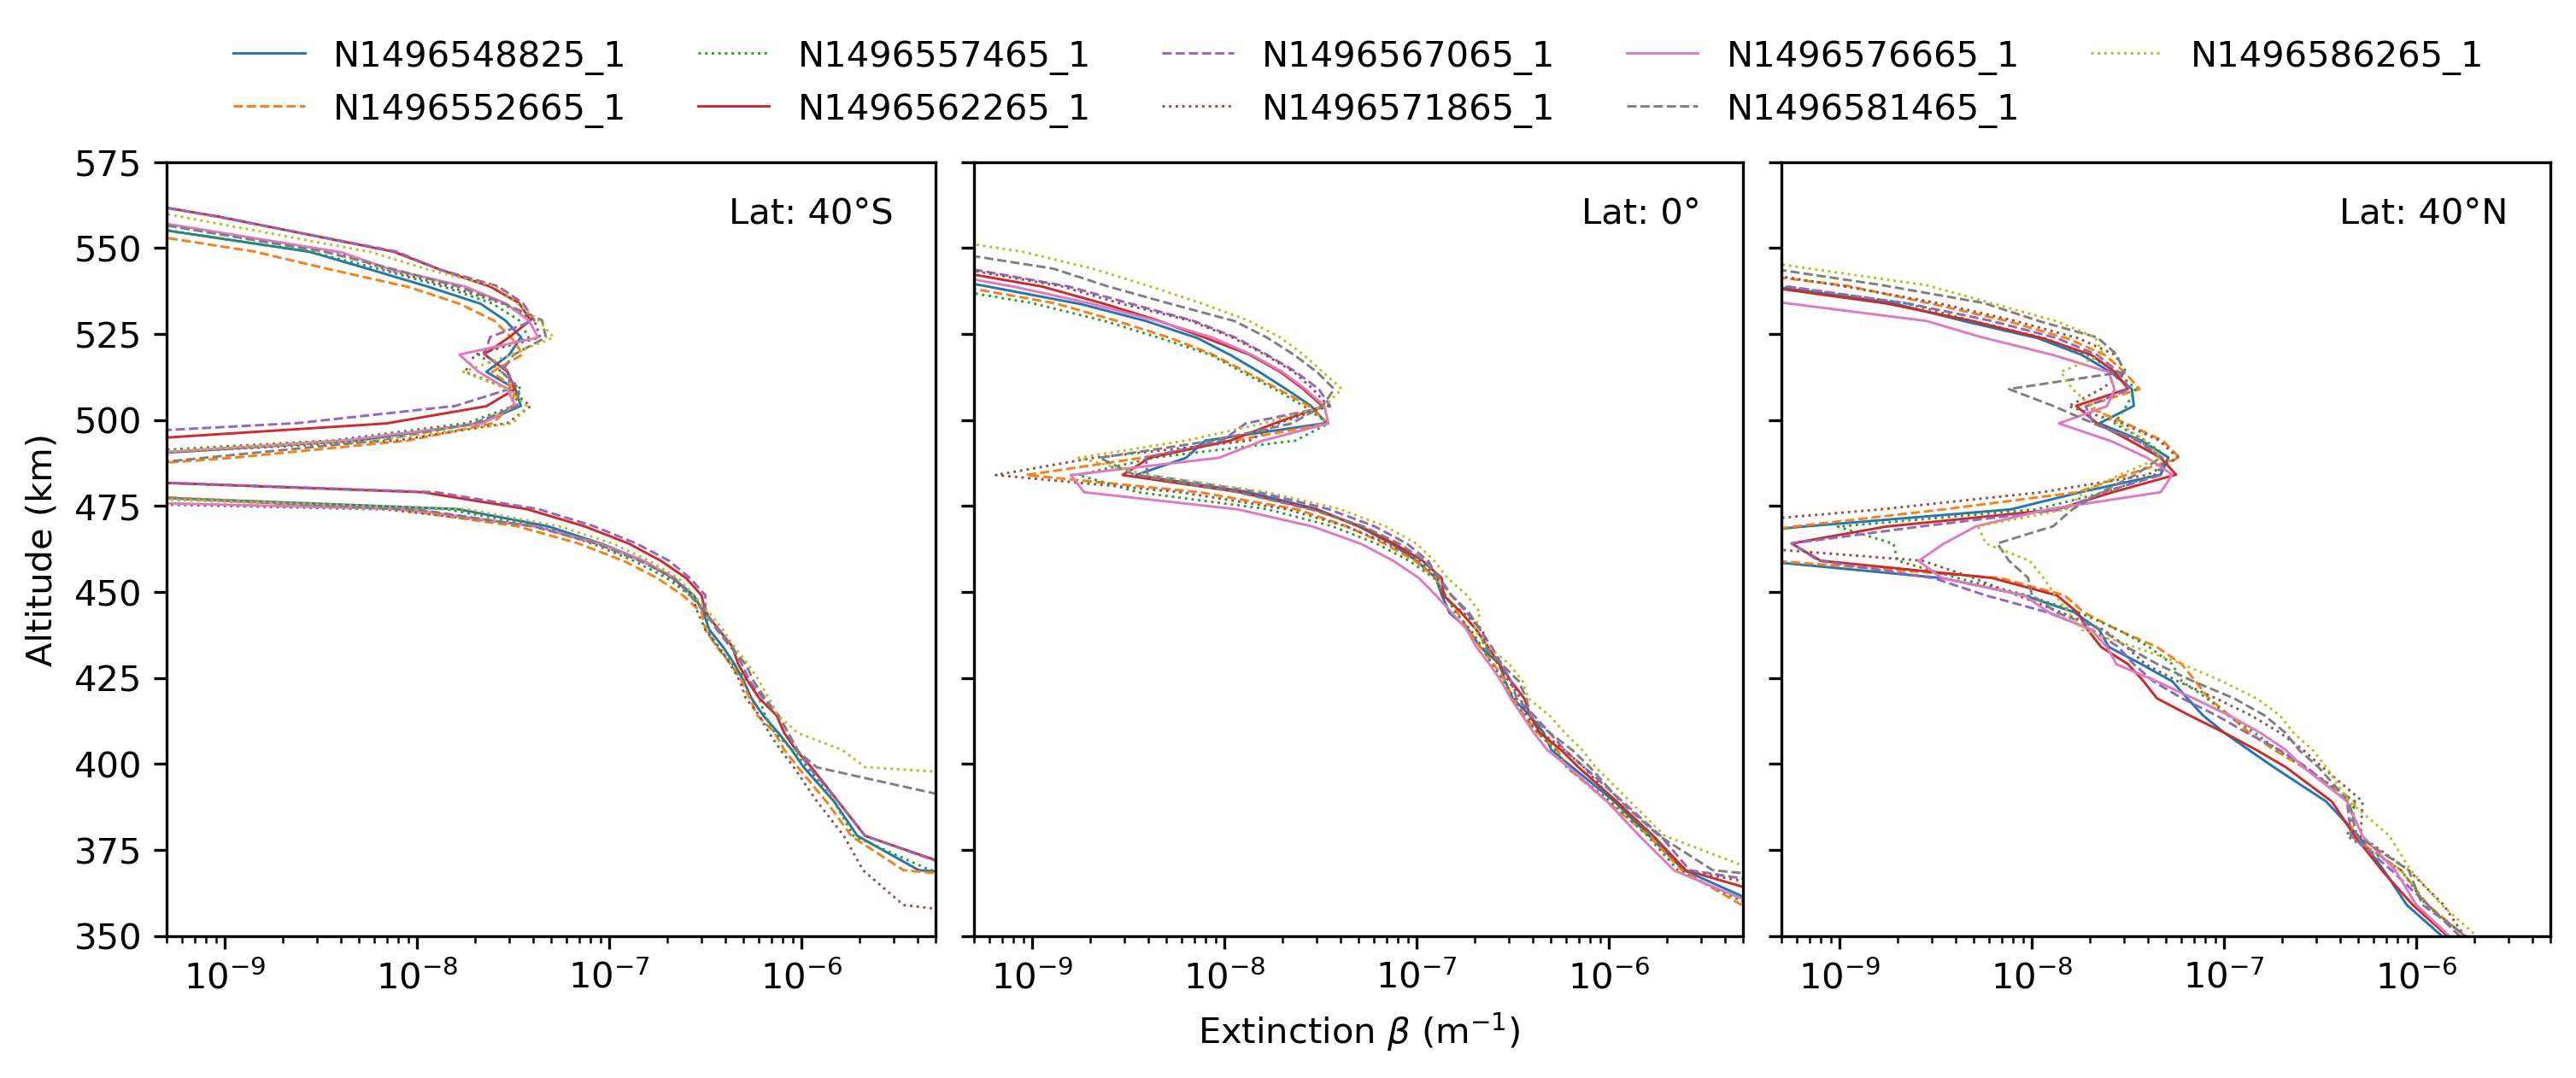
\includegraphics[width=\textwidth]{Fig/Time_variability.png}
    \caption{Extinction profiles for the series
    of 9 images taken 80 minutes apart in June 2005 (cf. Table \ref{tab:time_variability}).
    The global latitudinal map is shown in figure~\ref{fig:dhl_2004_2008}c.}
    \label{fig:time_variability}
\end{figure}

The figure~\ref{fig:time_variability} presents extinction profiles extracted from the analysis of these 9 images.
First, we confirm that our calibration method is reliable from one picture to the other and the overall
variability of the detached haze is very small. We clearly observe the double layering at \ang{40}S and \ang{40}N reported
previously. All the locations of the maximum of the extinction peaks are located within a small altitude range (smaller
than the 8 km of the pixel scale). Then, the vertical offsets which are observed at different times are consistent
with  the accuracy of the image navigation, and therefore are not significant. At the equator and at \ang{40}S, the detached
haze layer is well detached for all the profiles. When the vertical offset is accounter for, all the extinctions are found
with relative differences of about $\pm$ 10\% compared to the average value, except in the depletion zone between
the main and detached haze layers where difference can reach an order of magnitude (at \ang{0}) to several order of magnitude
(\ang{40}N). The variations outside the depletion zone are not significant. We note that the different behavior of the
N1496576665\_1 profile at \ang{40}S and below 450 km, compared to other profiles, is an artefact due to the inversion
process.

The variability in the depletion zone at the equator is probably due to the retrieval uncertainties. The differences in
extinction are about one order of magnitude, consistent with uncertainties between the two layers
\citep[\emph{e.g.}][]{West2018}, and without specific temporal evolution.
The variability observed at \ang{40}N, in the depletion zone around 460 km are significant for two reasons.
First, the differences are much larger than the expected uncertainty in this zone. Second, the sequence shows
a gradual and consistent increase of extinction with time. If these differences were due to uncertainties in
the retrieval procedure, it would have rather given a chaotic evolution of the extinction with time.

We also remark that the corresponding extinction map (Fig.~\ref{fig:dhl_2004_2008}c) shows that in the south,
the detached haze is well separated from the main haze by a well defined depletion zone. In the north, the depletion
zone is less well defined and the detached haze and the main haze are connected vertically by a residual haze.
The variation of this residual haze is the one reported in Fig.~\ref{fig:time_variability} at \ang{40}N.
We can not strictly determine if we are witnessing time or a spatial variations since both the time and the longitude
of the observations change simultaneously during the image sequence. We note that a rotation of \ang{5} in longitude
corresponds to a maximum shift of 250 km in distance (one tenth of Titan radius), possibly consistent with a spatial
variation of the haze extinction.
